\section{Internationale Arbeitsteilung}
\subsection{Komparativer Kostenvorteil}
\begin{multicols}{2}
	Vorgehen:
	\begin{itemize}
		\item Opportunitätskosten Berechnen für alle Artikel.
		\item Opportunitätskosten vergleichen.
		\item Der Ort mit den tiefsten Opportunitätskosten produziert und
		exportiert zu einem Preis zwischen Opportunitätskosten im
		Exportort und den Opportunitätskosten im Importort (natürlich nur ohne
		Zölle, Transportkosten etc.).
	\end{itemize}
	Falls Gleichstand ist findet kein Handel statt.
	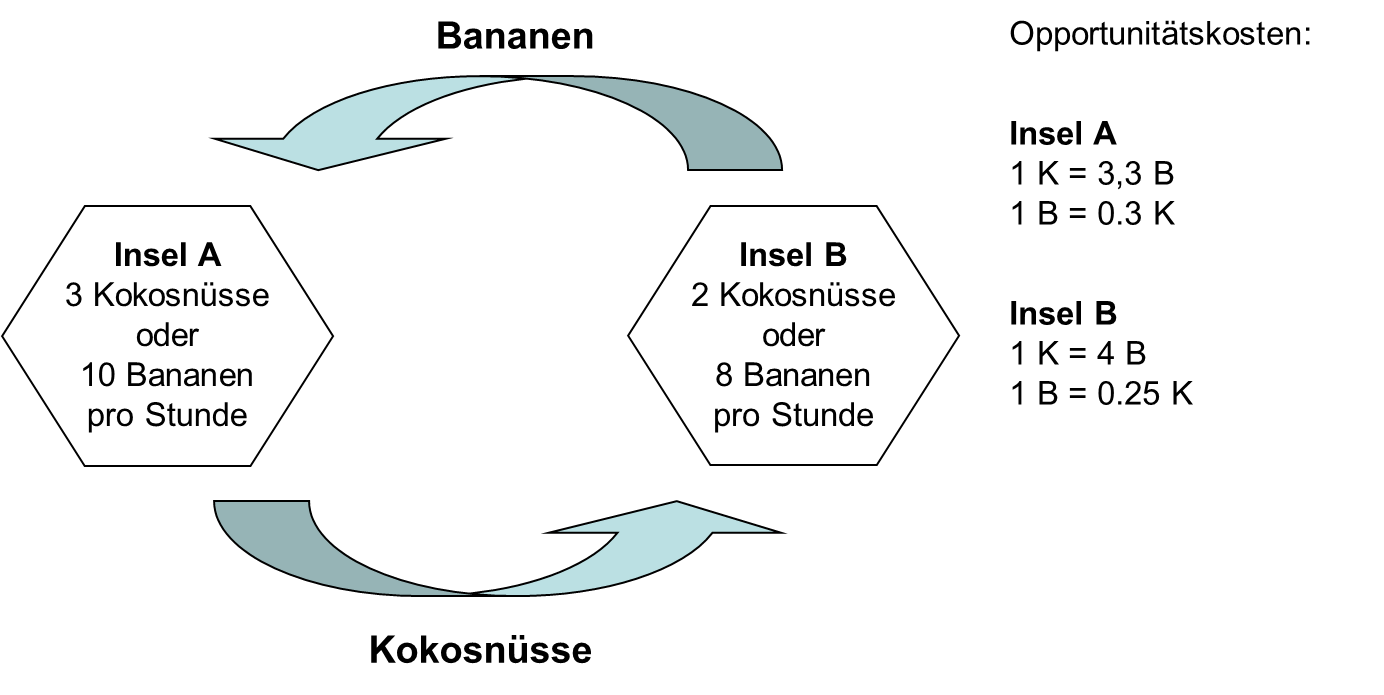
\includegraphics[width=9cm]{images/h03f07.png}
\end{multicols}
\subsection{Weltmarktpreis}
Hoher Weltmarktpreis: Konsument verliert, Allgemeinheit und Produktion gewinnt.\\
Tiefer Weltmarktpreis bewirkt genau das Gegenteil.\\
Internationale Arbeitsteilung bringt positive Wohlfahrtseffekte unabhängig
davon, ob der Weltmarktpreis höher oder tiefer als der Heimmarktpreis ist.
\begin{multicols}{2}
	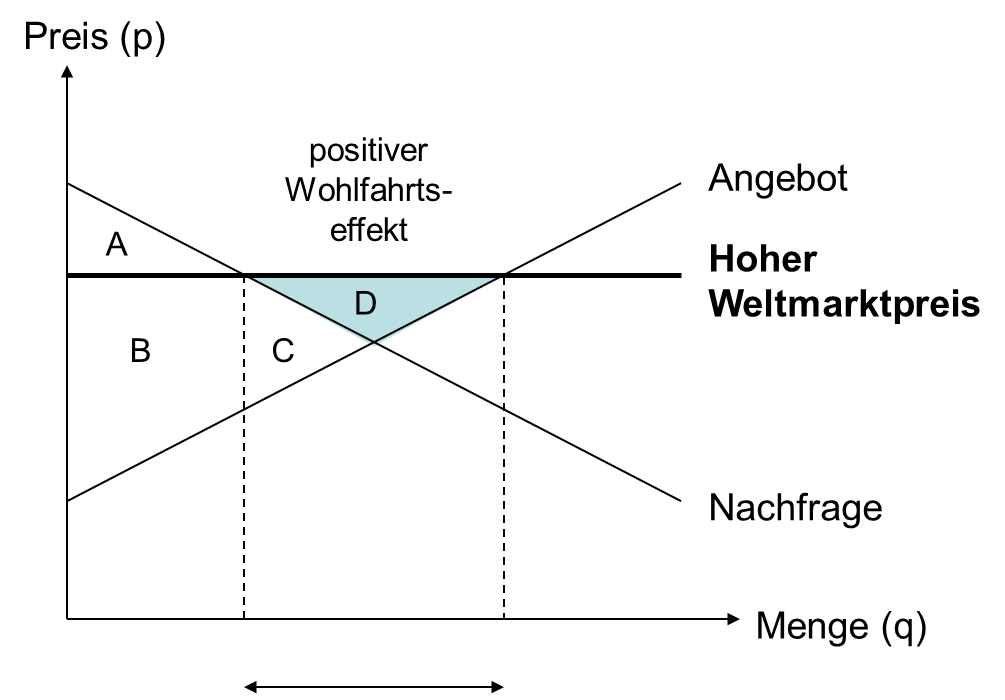
\includegraphics[width=9cm]{images/h03f11.png}\\
	\columnbreak\\
	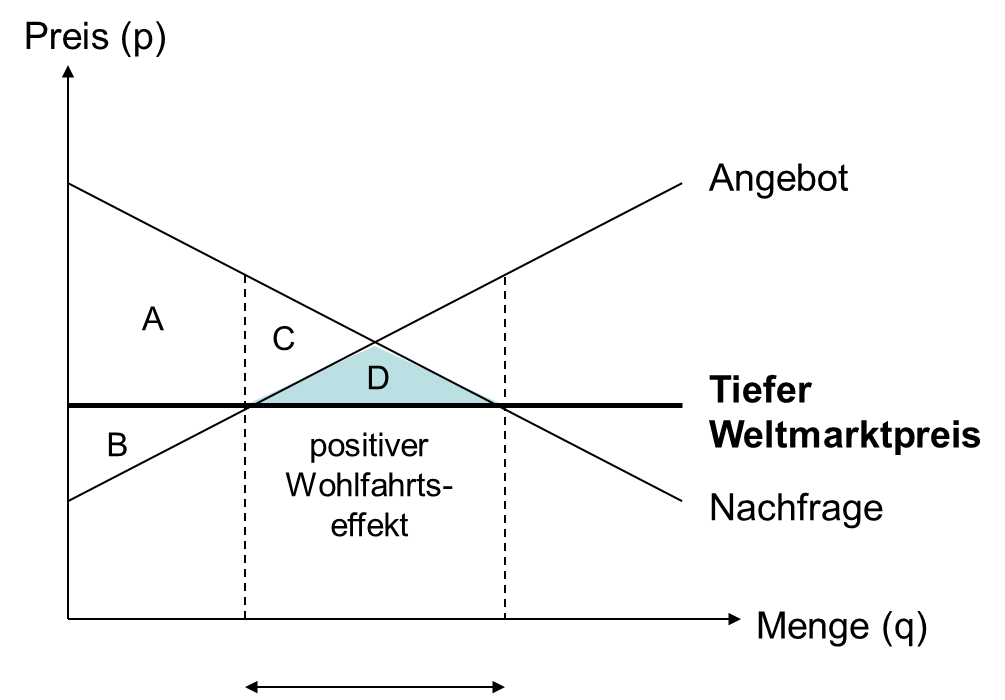
\includegraphics[width=9cm]{images/h03f13.png}
\end{multicols}
\subsection{Protektionismus (Zölle)}